% !TEX TS-program = pdflatex
% !TEX encoding = UTF-8 Unicode

% This file is a template using the "beamer" package to create slides for a talk or presentation
% - Giving a talk on some subject.
% - The talk is between 15min and 45min long.
% - Style is ornate.

% MODIFIED by Jonathan Kew, 2008-07-06
% The header comments and encoding in this file were modified for inclusion with TeXworks.
% The content is otherwise unchanged from the original distributed with the beamer package.

\documentclass{beamer}
\setbeamercovered{invisible}



% Copyright 2004 by Till Tantau <tantau@users.sourceforge.net>.
%
% In principle, this file can be redistributed and/or modified under
% the terms of the GNU Public License, version 2.
%
% However, this file is supposed to be a template to be modified
% for your own needs. For this reason, if you use this file as a
% template and not specifically distribute it as part of a another
% package/program, I grant the extra permission to freely copy and
% modify this file as you see fit and even to delete this copyright
% notice. 


\mode<presentation>
{
  \usetheme{Warsaw}
  % or ...

  % or whatever (possibly just delete it)
}


\usepackage[english]{babel}
% or whatever

\usepackage[utf8]{inputenc}
\usepackage{qrcode}
\usepackage{hyperref}
\usepackage{ytableau}
\usepackage{tikz}
% or whatever

\usepackage{times}
\usepackage[T1]{fontenc}
% Or whatever. Note that the encoding and the font should match. If T1
% does not look nice, try deleting the line with the fontenc.

%%% MATH RELATED
\newcommand{\N}{\mathbb{N}}
\newcommand{\Z}{\mathbb{Z}}
\newcommand{\R}{\mathbb{R}}
\newcommand{\pow}{\mathcal{P}}


% All Venn diagrams are editable TikZ artwork.
\newcommand{\vennbase}{
 \draw[thick] (-2.7,-1.65) rectangle (2.7,1.65);
 \draw[thick] (-.8,0) circle (1.2);
 \draw[thick] (.8,0) circle (1.2);
 \node at (-1.45,1.25) {$A$}; \node at (1.45,1.25) {$B$};
 \node at (-2.4,1.38) {$U$};}
\newcommand{\venn}[1]{\begin{tikzpicture}[scale=.9]
 \ifcase#1\relax
 \or \fill[blue!25] (-.8,0) circle (1.2);\fill[blue!25] (.8,0) circle (1.2);
 \or \begin{scope}\clip (-.8,0) circle (1.2);\fill[blue!35] (.8,0) circle (1.2);\end{scope}
 \or \fill[blue!30] (-.8,0) circle (1.2);\begin{scope}\clip (.8,0) circle (1.2);\fill[white] (-.8,0) circle (1.2);\end{scope}
 \or \fill[blue!25] (-2.7,-1.65) rectangle (2.7,1.65);\fill[white] (-.8,0) circle (1.2);
 \or \fill[blue!25] (-2.7,-1.65) rectangle (2.7,1.65);\fill[white] (-.8,0) circle (1.2);\fill[white] (.8,0) circle (1.2);
 \or \fill[blue!25] (-2.7,-1.65) rectangle (2.7,1.65);\begin{scope}\clip (-.8,0) circle (1.2);\fill[white] (.8,0) circle (1.2);\end{scope}
 \fi
 \vennbase
 \end{tikzpicture}}
\newcommand{\histsource}[2]{\par\medskip{\tiny Source: \href{#1}{#2}.\par}}

\title{MATH 180 Strategies of Problem Solving} 
\subtitle
{} % (optional)

\author[W.R. Casper] % (optional, use only with lots of authors)
{W.R. Casper}
% - Use the \inst{?} command only if the authors have different
%   affiliation.

\institute[California State University Fullerton] % (optional, but mostly needed)
{
  Department of Mathematics\\
  California State University Fullerton}
% - Use the \inst command only if there are several affiliations.
% - Keep it simple, no one is interested in your street address.

\subject{Talks}
% This is only inserted into the PDF information catalog. Can be left
% out. 



% If you have a file called "university-logo-filename.xxx", where xxx
% is a graphic format that can be processed by latex or pdflatex,
% resp., then you can add a logo as follows:

% \pgfdeclareimage[height=0.5cm]{university-logo}{university-logo-filename}
% \logo{\pgfuseimage{university-logo}}



% Delete this, if you do not want the table of contents to pop up at
% the beginning of each subsection:
\AtBeginSubsection[]
{
  \begin{frame}<beamer>{Outline}
    \tableofcontents[currentsection,currentsubsection]
  \end{frame}
}


% If you wish to uncover everything in a step-wise fashion, uncomment
% the following command: 

%\beamerdefaultoverlayspecification{<+->}


\begin{document}

\begin{frame}
  \titlepage
\end{frame}

\begin{frame}{Outline}
  \tableofcontents
  % You might wish to add the option [pausesections]
\end{frame}

% Since this a solution template for a generic talk, very little can
% be said about how it should be structured. However, the talk length
% of between 15min and 45min and the theme suggest that you stick to
% the following rules:  

% - Exactly two or three sections (other than the summary).
% - At *most* three subsections per section.
% - Talk about 30s to 2min per frame. So there should be between about
%   15 and 30 frames, all told.

\section{SoPS Lecture 17}
\subsection{Objects and statements}
\begin{frame}{What are we learning to do?}
\begin{block}{Our questions}
\begin{itemize}
\item What objects does an expression describe?
\item Does a sentence make mathematical sense?
\item If it makes sense, is it true?
\item How can we justify our answer?
\end{itemize}
\end{block}\medskip A false statement can still make perfectly good mathematical sense.
\end{frame}
\begin{frame}{A first sorting puzzle}
You know ordinary arithmetic. Classify each line.\[2+3=5\qquad 2+3=8\qquad 2+3\qquad 2+{}=5\]\begin{block}{Four possible responses}
\begin{itemize}
\item A meaningful true statement.
\item A meaningful false statement.
\item A meaningful expression, but no claim to evaluate.
\item An incomplete or undefined expression.
\end{itemize}
\end{block}
\end{frame}
\begin{frame}{A first sorting puzzle --- discussion}
\begin{itemize}
\item $2+3=5$ is a true statement.
\item $2+3=8$ is a false statement.
\item $2+3$ names a number. It makes sense, but is not a statement.
\item $2+{}=5$ is incomplete as written. We could repair it by introducing a variable.
\end{itemize}\begin{block}{One more possibility}
$x+3=5$ is an \textbf{open sentence}. Its truth depends on $x$.
\end{block}
\end{frame}
\begin{frame}{Sets}
\begin{block}{Working description}
A \textbf{set} is a collection of distinct objects, called its \textbf{elements} or \textbf{members}.
\end{block}\begin{itemize}
\item $A=\{1,2,3\}$ is a set of numbers.
\item $V=\{a,e,i,o,u\}$ is a set of letters.
\item A set can contain game positions, people, or other sets.
\end{itemize}\medskip We must be able to determine what counts as an element.
\end{frame}
\begin{frame}{Membership}
Let $A=\{1,2,3\}$.
\[2\in A\quad\text{means that 2 is an element of }A.\]
\[5\notin A\quad\text{means that 5 is not an element of }A.\]
\begin{block}{Reading aloud}
Read $\in$ as ``is an element of.'' This helps distinguish membership from other relationships.
\end{block}
\end{frame}
\begin{frame}{Which lines make sense?}
Let $A=\{1,2,3\}$. We use numbers as ordinary numbers.
\begin{block}{Discuss with a partner}
\begin{itemize}
\item $2\in A$
\item $5\in A$
\item $A+2=5$
\item $A$
\end{itemize}
\end{block}
\end{frame}
\begin{frame}{Which lines make sense? --- discussion}
Let $A=\{1,2,3\}$. We use numbers as ordinary numbers.
\begin{itemize}
\item $2\in A$: meaningful and true.
\item $5\in A$: meaningful and false.
\item $A+2=5$: we have not defined addition of a set and a number.
\item $A$: a meaningful name for a set, but no statement.
\end{itemize}
\end{frame}
\begin{frame}{Conventions matter}
\begin{block}{Our convention}
Numbers and letters are ordinary objects. We do not use a special set-theoretic encoding of numbers.
\end{block}\begin{itemize}
\item Expressions like $2\subseteq A$ will be undefined in our language, because $2$ is not being treated as a set.
\item Set membership $x\in A$ requires $A$ to be a set. The object $x$ may itself be a set.
\item An unfamiliar but well-defined expression may be false. Unfamiliarity alone does not make it meaningless.
\end{itemize}
\end{frame}

\subsection{Describing sets}
\begin{frame}{Order and repetition}
\[\{1,2,3\}=\{3,1,2\}=\{1,1,2,3,3\}.\]\begin{block}{Equality of sets}
Two sets are equal exactly when they have the same elements.
\end{block}\begin{itemize}
\item Order does not matter.
\item Listing an element again does not create another element.
\end{itemize}\medskip A set of dice outcomes and a sequence of dice rolls record different information.
\end{frame}
\begin{frame}{The same set?}
For each proposed equality, decide whether it is true.
\begin{block}{Discuss with a partner}
\begin{itemize}
\item $\{2,4,6\}=\{6,2,4\}$
\item $\{1,1,2\}=\{1,2,2\}$
\item $\{1,2\}=\{3\}$
\item $\{1,2\}=3$
\end{itemize}
\end{block}
\end{frame}
\begin{frame}{The same set? --- discussion}
For each proposed equality, decide whether it is true.
\begin{itemize}
\item True: the elements are identical.
\item True: each side has exactly the elements $1$ and $2$.
\item False: $1$ belongs to the left side and not the right.
\item False under our convention: a two-element set is not the number $3$. Equality can compare objects of different kinds.
\end{itemize}
\end{frame}
\begin{frame}{Set-builder notation}
\[E=\{x\in\Z:x\text{ is even}\}.\]\begin{itemize}
\item $x\in\Z$ specifies the allowed objects.
\item The colon means ``such that.
\item The condition selects which allowed objects belong.
\end{itemize}\begin{block}{Finite example}
$\{x\in\Z:0<x<5\}=\{1,2,3,4\}$.
\end{block}
\end{frame}
\begin{frame}{Some familiar infinite sets}
\[\begin{aligned}\N&=\{1,2,3,\ldots\},\\\Z&=\{\ldots,-2,-1,0,1,2,\ldots\},\\\mathbb Q&=\{a/b:a,b\in\Z,\ b\ne0\},\\\R&=\text{the set of real numbers}.\end{aligned}\]\medskip In these slides, $0\notin\N$. Some books use a different convention.\medskip\par Infinite sets need a description that specifies every element.
\end{frame}
\begin{frame}{Reading a set description}
Let $B=\{x\in\Z:x^2<10\}$.
\begin{block}{Discuss with a partner}
\begin{itemize}
\item List all elements of $B$.
\item Is $\sqrt2\in B$?
\item Is $-3\in B$?
\item Is $\{x\in\Z:x^2\}$ a complete set description?
\end{itemize}
\end{block}
\end{frame}
\begin{frame}{Reading a set description --- discussion}
Let $B=\{x\in\Z:x^2<10\}$.
\begin{itemize}
\item $B=\{-3,-2,-1,0,1,2,3\}$.
\item No. $\sqrt2$ fails the requirement $x\in\Z$.
\item Yes, because $(-3)^2=9<10$.
\item No. $x^2$ is a number, not a condition to test.
\end{itemize}
\end{frame}
\begin{frame}{Conditions versus output expressions}
\[\{x\in\Z:x^2<10\}\qquad\{x^2:x\in\Z\}\]\begin{itemize}
\item The first selects integers satisfying a condition.
\item The second collects the outputs $x^2$ for all integers $x$.
\item The second set is $\{0,1,4,9,16,\ldots\}$.
\end{itemize}\begin{block}{Check}
Why does the second set contain $9$ only once, even though $3^2=(-3)^2$?
\end{block}
\end{frame}
\subsection{Subsets and the empty set}
\begin{frame}{Subsets}
\begin{block}{Definition}
$A\subseteq B$ means that \textbf{every element of $A$ is also an element of $B$}.
\end{block}\[\{1,3\}\subseteq\{1,2,3\}.\]\begin{itemize}
\item $A\subseteq A$ for every set $A$.
\item $A\subsetneq B$ means $A\subseteq B$ and $A\ne B$.
\item We use $\subseteq$ to allow equality and $\subsetneq$ to exclude it.
\end{itemize}\medskip The symbol $\subset$ has different conventions in different books.
\end{frame}
\begin{frame}{Membership versus inclusion}
Let $A=\{1,2,3\}$.\[2\in A\qquad\{2\}\subseteq A.\]\begin{block}{What are we comparing?}
\begin{itemize}
\item $x\in A$ asks whether $x$ is one of the elements of $A$.
\item $B\subseteq A$ asks whether every element of $B$ belongs to $A$.
\end{itemize}
\end{block}\medskip $\{2\}$ is a set with one element. Its element is $2$.
\end{frame}
\begin{frame}{Membership or subset?}
Let $A=\{1,2,3\}$. Classify each line.
\begin{block}{Discuss with a partner}
\begin{itemize}
\item $1\in A$ and $\{1\}\in A$
\item $\{1\}\subseteq A$ and $A\subseteq A$
\item $1\subseteq A$
\item $A\in A$
\end{itemize}
\end{block}
\end{frame}
\begin{frame}{Membership or subset? --- discussion}
Let $A=\{1,2,3\}$. Classify each line.
\begin{itemize}
\item True and false, respectively. The elements of $A$ are numbers.
\item Both true.
\item Undefined in our convention: the left side must be a set.
\item Meaningful and false. None of the listed elements is $A$.
\end{itemize}
\end{frame}
\begin{frame}{The empty set}
\begin{block}{Definition}
The \textbf{empty set}, written $\varnothing$ or $\{\}$, has no elements.
\end{block}\[\{x\in\R:x^2=-1\}=\varnothing.\]\begin{itemize}
\item $\varnothing$ is a set.
\item $\{\varnothing\}$ has one element: the empty set.
\item $\varnothing\ne\{\varnothing\}$.
\end{itemize}\begin{block}{Question}
Is a box containing one empty box itself empty?
\end{block}
\end{frame}
\begin{frame}{Why the empty set is a subset of every set}
For any set $A$,\[\varnothing\subseteq A.\]\begin{block}{Reason}
To disprove this, we would need an element of $\varnothing$ that fails to belong to $A$. There is no element of $\varnothing$ at all.
\end{block}\medskip This is an example of \textbf{vacuous truth}.\medskip\par ``Every dragon in this room wears a hat is true if there are no dragons in this room.
\end{frame}
\begin{frame}{Empty-set check}
Let $A=\{1,2\}$.
\begin{block}{Discuss with a partner}
\begin{itemize}
\item $\varnothing\subseteq A$
\item $\varnothing\in A$
\item $\varnothing\in\{\varnothing\}$
\item $\{\varnothing\}\subseteq A$
\end{itemize}
\end{block}
\end{frame}
\begin{frame}{Empty-set check --- discussion}
Let $A=\{1,2\}$.
\begin{itemize}
\item True: the empty set is a subset of every set.
\item False: the only elements of $A$ are $1$ and $2$.
\item True: it is the one listed element.
\item False: this would require $\varnothing\in A$.
\end{itemize}
\end{frame}

\subsection{Sets containing sets}
\begin{frame}{Sets can be elements}
Let\[C=\{1,\{2,3\},\varnothing\}.\]\begin{itemize}
\item The elements of $C$ are $1$, $\{2,3\}$, and $\varnothing$.
\item $\{2,3\}\in C$ is true.
\item $2\in C$ is false.
\item $\{2,3\}\subseteq C$ is false.
\end{itemize}\begin{block}{Braces are structure}
A set containing a set does not automatically contain the elements of that inner set.
\end{block}
\end{frame}
\begin{frame}{Braces change the answer}
Let $D=\{1,\{1\},\{2,3\}\}$.
\begin{block}{Discuss with a partner}
\begin{itemize}
\item $1\in D$ and $\{1\}\in D$
\item $\{1\}\subseteq D$
\item $\{\{1\}\}\subseteq D$
\item $\{2,3\}\subseteq D$
\end{itemize}
\end{block}
\end{frame}
\begin{frame}{Braces change the answer --- discussion}
Let $D=\{1,\{1\},\{2,3\}\}$.
\begin{itemize}
\item Both true: both objects occur in the list.
\item True: its only element, $1$, belongs to $D$.
\item True: its only element, $\{1\}$, belongs to $D$.
\item False: neither $2$ nor $3$ is an element of $D$.
\end{itemize}
\end{frame}
\begin{frame}{A relation between the two symbols}
\begin{block}{Always true}
For every object $x$ and every set $A$,\[x\in A\quad\Longleftrightarrow\quad\{x\}\subseteq A.\]
\end{block}\begin{itemize}
\item The only element of $\{x\}$ is $x$.
\item So checking every element of $\{x\}$ means checking $x$.
\end{itemize}\begin{block}{Careful}
This does not say $x\in A$ is equivalent to $\{x\}\in A$.
\end{block}
\end{frame}
\begin{frame}{A short group challenge}
Construct a set $A$ satisfying each request separately.\begin{itemize}
\item $1\in A$ but $\{1\}\notin A$.
\item $\{1\}\in A$ but $1\notin A$.
\item Both $1\in A$ and $\{1\}\in A$.
\item $\varnothing\in A$ and $A$ has exactly two elements.
\end{itemize}\medskip Compare constructions. Can different groups give different correct answers?
\end{frame}
\begin{frame}{A short group challenge --- examples}
\begin{itemize}
\item $A=\{1\}$.
\item $A=\{\{1\}\}$.
\item $A=\{1,\{1\}\}$.
\item $A=\{\varnothing,7\}$.
\end{itemize}\begin{block}{Another check}
Why does $\{\varnothing,\varnothing\}$ fail?
\end{block}\medskip It has only one element. Repetition does not count.
\end{frame}
\section{Set algebra}
\subsection{Union, intersection, and difference}
\begin{frame}{Union and intersection}
For sets $A$ and $B$,\[\begin{aligned}A\cup B&=\{x:x\in A\text{ or }x\in B\},\\A\cap B&=\{x:x\in A\text{ and }x\in B\}.\end{aligned}\]\begin{block}{The mathematical word or}
An element belongs to $A\cup B$ if it belongs to either set \textbf{or to both}.
\end{block}\medskip Example: if $A=\{1,2,3\}$ and $B=\{3,4\}$,\[A\cup B=\{1,2,3,4\},\qquad A\cap B=\{3\}.\]
\end{frame}
\begin{frame}{Reading a Venn diagram}
\begin{center}\venn{0}\end{center}
The rectangle is the universe $U$. The circles represent sets $A$ and $B$.
\medskip\par Each position represents a possible element. The overlap represents elements belonging to both sets.
\end{frame}
\begin{frame}{Union in a Venn diagram}
\begin{center}\venn{1}\end{center}
\[x\in A\cup B\quad\Longleftrightarrow\quad x\in A\text{ or }x\in B.\]
The shaded region includes the overlap. Mathematical ``or'' allows both.
\end{frame}
\begin{frame}{Intersection in a Venn diagram}
\begin{center}\venn{2}\end{center}
\[x\in A\cap B\quad\Longleftrightarrow\quad x\in A\text{ and }x\in B.\]
\textbf{Check:} Does a point in $A$ but outside $B$ belong to the shaded set?
\end{frame}

\begin{frame}{Difference and complement}
\[A\setminus B=\{x\in A:x\notin B\}.\]If $A=\{1,2,3\}$ and $B=\{3,4\}$,\[A\setminus B=\{1,2\},\qquad B\setminus A=\{4\}.\]\begin{block}{Complement needs a universe}
If all objects under discussion lie in a fixed set $U$, then\[A^c=U\setminus A.\]Without a specified or understood $U$, the complement is ambiguous.
\end{block}
\end{frame}
\begin{frame}{Difference in a Venn diagram}
\begin{center}\venn{3}\end{center}
\[A\setminus B=\{x\in A:x\notin B\}.\]
\textbf{Check:} Where would we shade $B\setminus A$ instead?
\end{frame}
\begin{frame}{Complement in a Venn diagram}
\begin{center}\venn{4}\end{center}
The shaded region is $A^c=U\setminus A$.
\medskip\par \textbf{Check:} Why does part of $B$ belong to $A^c$, while another part does not?
\end{frame}

\begin{frame}{Calculating with sets}
Let $U=\{1,2,3,4,5,6\}$, $A=\{1,2,4\}$, $B=\{2,3,4\}$.
\begin{block}{Discuss with a partner}
\begin{itemize}
\item Find $A\cup B$ and $A\cap B$.
\item Find $A\setminus B$ and $B\setminus A$.
\item Find $A^c$.
\item Is $A\cap B=2$ true?
\end{itemize}
\end{block}
\end{frame}
\begin{frame}{Calculating with sets --- discussion}
Let $U=\{1,2,3,4,5,6\}$, $A=\{1,2,4\}$, $B=\{2,3,4\}$.
\begin{itemize}
\item $A\cup B=\{1,2,3,4\}$ and $A\cap B=\{2,4\}$.
\item $A\setminus B=\{1\}$ and $B\setminus A=\{3\}$.
\item $A^c=\{3,5,6\}$.
\item False. The intersection is a set, not the number of its elements.
\end{itemize}
\end{frame}
\begin{frame}{Which expressions mean something?}
Let $A=\{1,2\}$ and $B=\{2,3\}$.
\begin{block}{Discuss with a partner}
\begin{itemize}
\item $A\cup B$
\item $A\cup 2$
\item $2\in A\cap B$
\item $A\in B\cup\{A\}$
\end{itemize}
\end{block}
\end{frame}
\begin{frame}{Which expressions mean something? --- discussion}
Let $A=\{1,2\}$ and $B=\{2,3\}$.
\begin{itemize}
\item Meaningful set expression: $\{1,2,3\}$. No truth value by itself.
\item Undefined: union requires two sets in our convention.
\item Meaningful and true, since $A\cap B=\{2\}$.
\item Meaningful and true. The union has $A$ as an element.
\end{itemize}
\end{frame}
\begin{frame}{Venn diagram check}
\begin{center}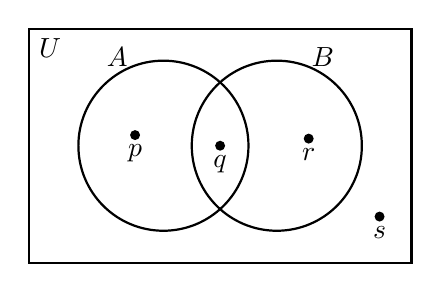
\begin{tikzpicture}[scale=.9]
\vennbase
\fill (-1.2,.15) circle (2pt) node[below] {$p$};
\fill (0,0) circle (2pt) node[below] {$q$};
\fill (1.25,.1) circle (2pt) node[below] {$r$};
\fill (2.25,-1) circle (2pt) node[below] {$s$};
\end{tikzpicture}\end{center}
Which points belong to $A\cup B$, $A\cap B$, $A\setminus B$, and $(A\cup B)^c$?
\medskip\par Are $p\in A$ and $p\subseteq A$ equally meaningful? Treat $p$ as a point, not a set.
\end{frame}
\begin{frame}{Venn diagram check --- answers}
\begin{center}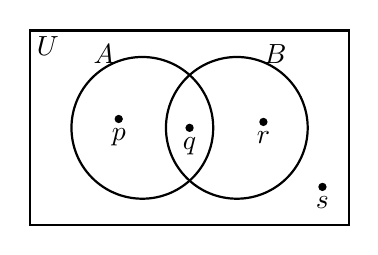
\begin{tikzpicture}[scale=.75]
\vennbase
\fill (-1.2,.15) circle (2pt) node[below] {$p$};
\fill (0,0) circle (2pt) node[below] {$q$};
\fill (1.25,.1) circle (2pt) node[below] {$r$};
\fill (2.25,-1) circle (2pt) node[below] {$s$};
\end{tikzpicture}\end{center}
Among the labeled points: $p,q,r$ belong to $A\cup B$, $q$ belongs to $A\cap B$, $p$ belongs to $A\setminus B$, and $s$ belongs to $(A\cup B)^c$.
\medskip\par $p\in A$ is true. We have not defined $p\subseteq A$ for a point.
\end{frame}

\begin{frame}{Disjoint sets}
\begin{block}{Definition}
Sets $A$ and $B$ are \textbf{disjoint} if $A\cap B=\varnothing$.
\end{block}\begin{itemize}
\item $\{1,3,5\}$ and $\{2,4,6\}$ are disjoint.
\item $\{1,2\}$ and $\{2,3\}$ are different but not disjoint.
\item $\{\varnothing\}$ and $\varnothing$ are disjoint.
\end{itemize}\begin{block}{Check}
Can a nonempty set be disjoint from itself? Explain.
\end{block}
\end{frame}
\begin{frame}{Inclusion and disjointness in pictures}
\begin{columns}[T]
\begin{column}{.49\textwidth}\centering
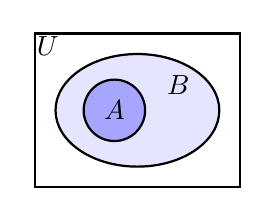
\begin{tikzpicture}[scale=.65]
\draw[thick] (-2,-1.5) rectangle (2,1.5);
\filldraw[fill=blue!10,thick] (0,0) ellipse (1.6 and 1.1);
\filldraw[fill=blue!35,thick] (-.45,0) circle (.6);
\node at (-.45,0) {$A$};\node at (.8,.5) {$B$};\node at (-1.75,1.25) {$U$};
\end{tikzpicture}\par $A\subseteq B$
\end{column}
\begin{column}{.49\textwidth}\centering
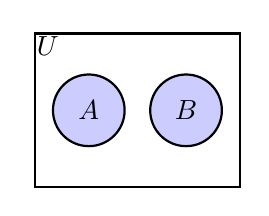
\begin{tikzpicture}[scale=.65]
\draw[thick] (-2,-1.5) rectangle (2,1.5);
\filldraw[fill=blue!20,thick] (-.95,0) circle (.7);
\filldraw[fill=blue!20,thick] (.95,0) circle (.7);
\node at (-.95,0) {$A$};\node at (.95,0) {$B$};\node at (-1.75,1.25) {$U$};
\end{tikzpicture}\par $A\cap B=\varnothing$
\end{column}\end{columns}
\medskip The left picture says every element of $A$ belongs to $B$.
\medskip\par It does not assert $A\in B$. Circles contain points representing elements, not automatically the circles themselves.
\end{frame}

\begin{frame}{Identities worth testing}
For arbitrary sets $A$ and $B$, which are always true?\begin{itemize}
\item $A\cup B=B\cup A$.
\item $A\cap B=B\cap A$.
\item $A\setminus B=B\setminus A$.
\item $A\cup\varnothing=A$ and $A\cap\varnothing=\varnothing$.
\end{itemize}\medskip For a false claim, find a small counterexample.
\end{frame}
\begin{frame}{Identities worth testing --- discussion}
\begin{itemize}
\item Union and intersection are commutative: the first two are true.
\item Difference need not be commutative. Take $A=\{1\}$ and $B=\{2\}$. Then $A\setminus B=\{1\}$ and $B\setminus A=\{2\}$.
\item Both empty-set identities are true.
\end{itemize}\begin{block}{A counterexample}
One example where a universal claim fails disproves that claim. Many successful examples do not prove it.
\end{block}
\end{frame}
\begin{frame}{De Morgan's laws}
With a fixed universe $U$,\[(A\cup B)^c=A^c\cap B^c,\qquad(A\cap B)^c=A^c\cup B^c.\]\begin{block}{Example in words}
``Not (plays chess or plays Go) means ``does not play chess and does not play Go.
\end{block}\medskip Test both identities with $U=\{1,2,3,4\}$, $A=\{1,2\}$, and $B=\{2,3\}$.
\end{frame}
\begin{frame}{De Morgan's laws in pictures}
\begin{columns}
\begin{column}{.49\textwidth}\centering\resizebox{\linewidth}{!}{\venn{5}}\par
$(A\cup B)^c=A^c\cap B^c$
\end{column}
\begin{column}{.49\textwidth}\centering\resizebox{\linewidth}{!}{\venn{6}}\par
$(A\cap B)^c=A^c\cup B^c$
\end{column}\end{columns}
\medskip\textbf{Left:} outside both circles.\par\textbf{Right:} everywhere except the overlap.
\medskip\par \textbf{Check:} In the right picture, why is the part belonging only to $A$ shaded?
\end{frame}

\begin{frame}{De Morgan's laws --- example}
Here $A^c=\{3,4\}$ and $B^c=\{1,4\}$.\[\begin{aligned}(A\cup B)^c&=\{1,2,3\}^c=\{4\},\\A^c\cap B^c&=\{3,4\}\cap\{1,4\}=\{4\},\\(A\cap B)^c&=\{2\}^c=\{1,3,4\},\\A^c\cup B^c&=\{3,4\}\cup\{1,4\}=\{1,3,4\}.\end{aligned}\]This verifies this example. A proof must work for every $x$ and every choice of $A,B$.
\end{frame}

\begin{frame}{Final thoughts}
  \begin{block}{Reflection}
\begin{itemize}
\item How do $x\in A$ and $\{x\}\subseteq A$ relate?
\item Why is $\varnothing\subseteq A$ always true?
\item Give a meaningful false statement and an undefined expression.
\item Find $\pow(\{\varnothing,1\})$.
\end{itemize}
  \end{block}
\begin{center}
Submit your responses by \textbf{Tonight!}
\end{center}
\end{frame}


\end{document}


